\documentclass[11pt]{article}
\title{Midterm 1 Prep}
%% Language and font encodings
\usepackage[english]{babel}
\usepackage[utf8x]{inputenc}
\usepackage[T1]{fontenc}

\usepackage{helvet}

%% Sets page size and margins
\usepackage[letterpaper,top=3cm,bottom=2cm,left=3cm,right=3cm,marginparwidth=1.75cm]{geometry}

%% Useful packages
\usepackage{amsmath}
\usepackage{graphicx}
\usepackage{tcolorbox}
\usepackage{amssymb}
\usepackage{amsthm}
\usepackage{lastpage}
\usepackage{accents}
\usepackage{multicol}

% For better list numbering
\usepackage[shortlabels]{enumitem}

% Font
% \usepackage{tgbonum}


% Tikz
\usepackage{tikz}

\usetikzlibrary{calc,fit,shapes.misc,backgrounds}
\usepackage{pgfplots}
\pgfplotsset{compat = newest}
\usetikzlibrary{positioning, arrows.meta}
\usepgfplotslibrary{fillbetween}

% Headers
\usepackage{fancyhdr}
\pagestyle{fancy}

% Store \@title as \thetitle
\makeatletter
\let\thetitle\@title
\makeatother

\fancyhf{}
\lhead{\fontfamily{qbk}\fontsize{10}{11}\selectfont ECON 3070}
\rhead{\fontfamily{qbk}\fontsize{10}{11}\selectfont \thetitle}
\rfoot{\fontfamily{qbk}\fontsize{10}{11}\selectfont \thepage}


% Sections and Subsections

% define colors
\definecolor{buff-gold}{HTML}{CFB87C}
\definecolor{buff-grey}{HTML}{565A5C}
% custom tcolorbox
\tcbset{colframe=buff-gold, colback=white!100!black}

% new page per section
\usepackage{titlesec}
\newcommand{\sectionbreak}{\clearpage}
% change style of section
\usepackage{sectsty}
\sectionfont{\color{buff-gold} \fontfamily{qbk}\selectfont}
\subsectionfont{\color{buff-grey} \fontfamily{qbk}\selectfont}


\newtoggle{INCLUDEANSWERS}
% \toggletrue{INCLUDEANSWERS}
\togglefalse{INCLUDEANSWERS}

\newcommand{\answer}[1]{\iftoggle{INCLUDEANSWERS}{{\color{violet!70!white}\textbf{Solution:} #1}}{}}


\begin{document}
  
\section*{Midterm 1 Prep}

\subsection*{Supply and Demand}
\begin{enumerate}
  \item The market for bike locks is described by the demand curve $P = 80 - Q_d$ and the supply curve $Q_s = 2P - 10 $. Answer the following questions:

    \begin{enumerate}
      \item When the price of bike locks is \$40 how many bike locks will be demanded? How many bike locks will be produced? Why would this not be the equilibrium price? Which way will the price move in this market.

      \item What is the marginal willingness to pay for the 40th bike lock? What is the marginal cost of the 40th unit?

      \item What is the market equilibrium values of price and quantity in the market of bike locks? 
    \end{enumerate}

    \answer{
      \begin{enumerate}
        \item $Q_d = 80 - P = 80 - 40 = 40$. $Q_s = 2P - 10 = 80 - 10 = 70$. This is not the equilibrium price since there is excess supply. The sellers will bid the price down.
        
        \item The marginal willingness to pay curve is given by demand, solving for $P$: $P = 80 - Q_d$. Similarly, the marginal cost curve is given by supply, solving for $P$: $P = Q_s/2 - 5$. In this case, the marginal willingness to pay is \$40 for the 40th unit and the marginal cost is \$15 for the 40th unit.
        
        \item $Q_d = 80 - P = 2P - 10 = Q_s$. This implies $3P = 90$, or $P^* = 30$. Plugging back into supply gives $Q_s = Q_d = 2*30 - 10 = 50$. Checking our work, we can plug into the demand curve and have $Q_d = 80 - 30 = 50$. 
      \end{enumerate}
    }

  \item The market contains two consumers $A$ and $B$ with the following demand functions: $Q_A^D = 40 - 5P$ and $Q_B^D = 18 - 5P$
  
  \begin{enumerate}
    \item Find the aggregate demand curve for this market. Draw this curve
    
    \answer{
      $$
        Q_{mkt}^D =
        \begin{cases}
          58 - 10P & \text{if } P \leq 4 \\
          40 - 5P & \text{if } 4 \leq P \leq 8 \\
          0       & \text{otherwise}.
        \end{cases}
      $$
    }
    
    \item Let market supply be given by $Q_{mkt}^S = 2P - 2$. Solve for the equilibrium quantity and price.
    
    \answer{
      Trying $P \leq 4$, 
      $$
        58 - 10P = 2P - 2 \implies P = 5
      $$
      This doesn't work because we assumed $P \leq 4$.

      Trying, $4 \leq P \leq 8$,
      $$
        40 - 5P = 2P - 2 \implies P = 6
      $$
      This works! Pluging back into supply, $Q_{mkt} = 2 * 6 - 2 = 10$. Checking our work, $Q_{mkt}^D = 40 - 5 * 6 = 10$. 
    }
  \end{enumerate}
\end{enumerate}

\subsection*{Supply/Demand Curve Shifters}
\begin{enumerate}
  \item For the following comparative static scenarios, describe what will happen the equilibrium price and quantity?
  
  \begin{enumerate}
    \item A stimulus check makes people richer
    \item A flood wipes out wheat crops in the midwest
    \item A flood wipes out crops in the midwest \emph{and} more people start getting into bread-making
  \end{enumerate}

  \answer{
    \begin{enumerate}
      \item Price goes up; quantity goes up
      
      \item Price goes up; quantity goes down
      
      \item Price goes up; quantity indeterminate
    \end{enumerate}
  }
\end{enumerate}


\subsection*{Elasticities}

\begin{enumerate}
  \item Suppose that when the price of the new macbook is \$1,600
  per tire, quantity demanded in Boulder is 40,000. Now suppose
  that the price has fallen to \$1,400, and the quantity demanded is
  50,000. What is the price elasticy of demand? Interpret this elasticity in words.

  \answer{
    $\% \Delta \text{ in } Q = (50,000 - 40,000) / 40,000 = 0.25$

    $\% \Delta \text{ in } P = (1,400 - 1,600) / 1,600 = -0.125$

    $$
    \frac{\% \Delta \text{ in } Q}{\% \Delta \text{ in } P} = \frac{0.25}{-0.125} = -2
    $$

    To interpret, we say a 1\% increase in price yields a 2\% decrease in quantity demanded.
  }

  \item A firm increases its price from \$8 to \$12 and sees demand for the product fall by 20\%. What would the price elasticity of demand be for this product?

  \answer{$(12 - 8)/8 = 0.5$. Therefore, $\varepsilon_{Q, P} = {0.2}{-0.5} = -0.4$. To interpret, we say that a 1\% increase in price yields a 0.4\% decrease in quantity demanded.}
  
  \item If disposable incomes rise by 5\% and demand changes from 100 units to 105, what is the income elasticity of demand? Interpret this number
  
  \answer{$(100 - 105)/100 = 5\%$. Therefore, $\varepsilon_{Q, I} = {5\%}{5\%} = 1$. To interpret, we say that a 1\% increase in income increases quantity demanded by 1\%.}
  
  \item What type of good would you expected to have a negative income elasticity of demand?
  
  \answer{Inferior good. $\frac{\partial x^*}{\partial I} < 0$}
\end{enumerate}


\subsection*{Utility Functions}
\begin{enumerate}
  \item For the following utility functions, solve for the marginal utility with respect to $x$. Interpret the marginal utility at $x = 3$. Is this utility diminishing as you increase $x$?
  \begin{enumerate}
    \item $U(x,y) = x^{1/3}y^{1/3}$
    \item $U(x,y) = 3x + 4y$
    \item $U(x,y) = x^{3/4}y^{1/4}$
  \end{enumerate}

  \item For the following utility functions, draw two indifference curves for these utility functions. 
  \begin{enumerate}
    \item $U(x,y) = x^{1/3}y^{1/3}$
    \item $U(x,y) = 3x + 4y$
    \item $U(x,y) = x^{3/4}y^{1/4}$
  \end{enumerate}

  \item In words, describe what an indifference curve is
  
  \item For the following utility functions, Calculate the marginal rate of substitution $MRS_{x,y}$. Interpret the marginal rate of substitution.
  \begin{enumerate}
    \item $U(x,y) = x^{1/3}y^{1/3}$
    \item $U(x,y) = 3x + 4y$
    \item $U(x,y) = x^{3/4}y^{1/4}$
  \end{enumerate}
\end{enumerate}


\subsection*{Budget Constraints}
\begin{enumerate}
  \item In words, write out the meaning of the budget constraint: 
  $$P_x x + P_y y = I$$

  \item Write out the budget constraint for $P_x = 10$, $P_y = 2$, and $I = 30$. Graph this curve.
  
  \item What happens to the above budget constraint for the following conditions:
  \begin{enumerate}
    \item $P_x$ moves to $\$5$
    \item $I$ goes up to $60$.
    \item $P_y$ drops to $\$1$.
  \end{enumerate}

  \item For which of the above conditions, will the consumer be better off? How do you know? 
\end{enumerate}


\subsection*{Optimality Conditions}
\begin{enumerate}
  \item In words, write out why we need the optimality condition to hold for optimal consumption:
  $$
    \frac{MU_x}{P_x} = \frac{MU_y}{P_y}
  $$

  \item For the following utility functions, write out the optimality condition
  \begin{enumerate}
    \item $U(x,y) = x^{1/3}y^{1/3}$
    \item $U(x,y) = 3x + 4y$
    \item $U(x,y) = x^{3/4}y^{1/4}$
  \end{enumerate}

  \item Write out the three main utility functions we have talked about in class. What are the optimality conditions for each of them?
\end{enumerate}


\subsection*{Optimal Demand}
\begin{enumerate}
  \item Interpret in words the optimization problem that consumers face:
  $$
    \max_{x,y} U(x,y) \text{ subject to } P_x x + P_y y = I
  $$

  \item What are the two things you need to solve for optimal demand?

  \item Solve the following problems for demand

  \begin{enumerate}
    \item $U(x,y) = \min(2x, y) \text{ and } P_x = 3, P_y = 1, I = 20$
    
    \item $U(x,y) = 2x + y \text{ and } P_x = 1, P_y = 3, I = 24$
    
    \item $U(x,y) = x^{\frac{2}{3}} y^{\frac{1}{3}}  \text{ and } P_x = 2, P_y = 2, I = 18$
  \end{enumerate}
\end{enumerate}

\subsection*{Consumption Curves}
\begin{enumerate}
  \item Solve for the demand functions $x^*(P_x, P_y, I)$ and $y^*(P_x, P_y, I)$ for the following utility functions:
  
  \begin{enumerate}
    \item $U(x,y) = x^{1/2} y^{1/2}$
    \item $U(x,y) = \min(x, 2y)$
    \item $U(x,y) = 2(x + y)$
  \end{enumerate}

  \item Solve for the demand functions $x^*(P_x, P_y, I)$ and $y^*(P_x, P_y, I)$ for $U(x,y) = x^{1/2} y^{1/2}$. Answer the following
  \begin{enumerate}
    \item What is the deriviative with respect to income, $I$? Does this imply the good is a normal good or a inferior good?
    
    \item Are $x$ and $y$ normal goods?
    
    \item Graph the demand curve $x^*(P_x)$ for $I = 12$ and $P_y = 4$ with $P_x$ on the $y$-axis and $x^*$ on the $x$-axis.
    
    \item Graph the engel curve $x^*(I)$ for $P_x = 4$ and $P_y = 2$ with $I$ on the $y$-axis and $x^*$ on the $x$-axis.
  \end{enumerate}
\end{enumerate}

\subsection*{Income and Substitution Effect}
\begin{enumerate}
  \item In words, describe what the income effect and the substitution effects are.
  
  \item Suppose that the price for good $x$ increases, show using the optimality condition, why you know that demand for $x$ must decrease. 
  
  \item How do you know if the income effect is positive or negative?

  \item For the below figure, highlight the income effect and the substitution effect. Is this good a normal good or an inferior good?
  
  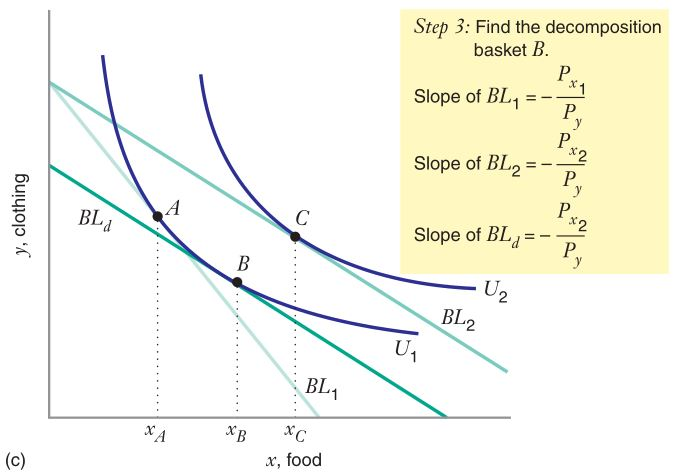
\includegraphics[width=0.6\linewidth]{../Lecture Slides/figures/fig5_6c.JPG}
\end{enumerate}

\subsection*{Consumer Welfare}
\begin{enumerate}
  \item If the demand for a product is $Q_D = 100 - 4P$, what is the consumer surplus generated when the market price is $P = 10$? Suppose a tax is imposed that raises the equilibrium price to $P = 12$. What is the new consumer surplus? What is the loss in consumer surplus from this tax?
  
  \item If the demand for a product is $Q_D = 144 - 12P$, what is the consumer surplus generated when the market price is $P = 6$? Suppose a subsidy is imposed that lowers the equilibrium price to $P = 4$. What is the new consumer surplus? What is the gains for consumers from this subsidy?
\end{enumerate}

\subsection*{Labor-Leisure}
\begin{enumerate}
  \item The current wage in Boulder is $12$. The consumer's utility function for labor, $L$, and the composite good $Y$ is given by $U(L, Y) = L^{1/2} Y^{1/2}$. 
  
  \begin{enumerate}
    \item Write out the budget constraint for leisure and the composite good.
    
    \item Solve for this consumer's optimal amount of hours worked, $24 - L$, and the amount of the composite good, $Y$, they consume.
    
    \item Now, suppose a minimum wage increases wages to $15$. Solve for hours worked and the amount of the composite good consumed.
  \end{enumerate}

  \item Say that the wage raised from \$15 to \$20 and the amount of labor supplied decreases. Explain why that could be possible.
\end{enumerate}
\end{document}
